%! Public Domain Software 2022-2025
%! 2025-08-27
%! 4.0.5-beta
%! Elayson Abreu
%! abntexto.classe@gmail.com

% !TeX TS-program = lualatex
\documentclass{abntexto}

% Precisamos do shorthands=off em babel para
% que o tikz-cd.sty funcione corretamente.

\usepackage{lipsum}
\usepackage[english,brazil,shorthands=off]{babel}
\usepackage[style=abnt]{biblatex} \addbibresource{abntexto-exemplo.bib}
\usepackage[colorlinks,linktocpage]{hyperref}
\usepackage{fontspec}
\usepackage{unicode-math}
\usepackage{multirow}
\usepackage{booktabs}
\usepackage{tikz}
\usepackage{chemfig}
\usepackage[siunitx]{circuitikz}
\usepackage{pseudo}
\usepackage{tikz-cd}
\usepackage[brazilian,noabbrev,capitalize]{cleveref} \AtBeginDocument{\def\ref{\cref}}

\setmainfont{XITS}[
    UprightFont    = *-Regular,
    BoldFont       = *-Bold,
    ItalicFont     = *-Italic,
    BoldItalicFont = *-BoldItalic,
    Extension      = .otf
]
\setmathfont{XITSMath-Regular.otf}
\setmonofont{InconsolataN-Regular.otf}

% Só é preciso guardar em macros informações que
% serão utilizadas repetidas vezes como o Nome ou
% o Título do trabalho, por exemplo.

\def \Autor{Elayson Abreu}
\def \Instituicao{Instituição}
\def \IniciaisDaInstituicao{SIGLA}
\def \Cidade{Cidade}
\def \AnoDeEntrega{Ano}
\def \Titulo{Classe {\ttfamily abntexto} para \LaTeX\ versão 4.0.5-beta: um exemplo de uso}
\def \TipoDeTrabalho{Dissertação}
\def \DescricaoDoTrabalho{\TipoDeTrabalho\ apresentada a \Instituicao\ como cumprimento às exigências legais para obtenção do título de Mestre.}
\def \AreaDeConcentracao{Matemática}
\def \Orientador{Dr.\,Nome}
\def \Coorientador{Dr.\,Nome}

\definelegendplace{g}{Gráfico}{logr}
\definelegendplace{c}{Composto}{loq}
\definelegendplace{circ}{Circuito}{locirc}
\definelegendplace{a}{Algoritmo}{loa}
\definelegendplace{d}{Diagrama}{lod}
\definelegendplace{f}{Fotografia}{lof}
\Crefname{g}{Gráfico}{Gráficos}
\Crefname{c}{Composto}{Compostos}
\Crefname{circ}{Circuito}{Circuitos}
\Crefname{a}{Algoritmo}{Algoritmos}
\Crefname{d}{Diagrama}{Diagramas}
\Crefname{f}{Fotografia}{Fotografias}

\def\savednote{}
\appto\resetplace{\global\let\savednote=\empty}
\long\def\note#1{\def\savednote{#1}}
\def\notelabel{Nota:~}
\def\printnotebox{\par\nointerlineskip \nobreak\vskip\medskipamount
    \hfil \vbox{\hsize=\savedplacewidth
        \raggedright\abntsmall\singlesp
        \setbox0=\hbox{\notelabel}%
        \leftskip=\wd0 \hskip-\wd0 \notelabel \savednote \strut
}}
\appto\printsrcbox{%
    \ifx\savednote\empty \else \printnotebox \fi
}

\let\onesidelayout=\eletroniclayout
\let\twosidelayout=\eletroniclayout
\def\Centro{\noindent\hfil}
\def\Direita{\noindent\hfill}
\def\me{Elaboração própria.}
\def\bibfont{\raggedright\interlinepenalty=10000\singlesp\bibitemsep=\baselineskip}
\hypersetup{
    pdfauthor   = \Autor,
    pdftitle    = \Titulo,
    pdfcreator  = LaTeX with abntexto,
    pdfkeywords = P1. P2. P3. P4,
}
\makeatletter



\begin{document}

% CAPA
% ================================================

\Centro
\begin{minipage}{.7\linewidth}
    \centering
    \includegraphics[height=4\baselineskip]{example-image}\\
    \Instituicao
\end{minipage}
\Enter[7]

\Centro\Autor
\Enter[3]

\Centro
\begin{minipage}{.7\linewidth}
    \centering
    \Titulo
\end{minipage}
\vfill

\Centro\Cidade % A próxima linha em branco é necessária.

\Centro\AnoDeEntrega

\newpage

% FOLHA DE ROSTO
% ================================================

\Centro\Autor
\Enter[9]

\Centro
\begin{minipage}{.7\linewidth}
    \centering
    \Titulo
\end{minipage}
\Enter[2]

\Direita
\begin{minipage}{.5\linewidth}
    \singlesp\nohyph
    \DescricaoDoTrabalho\Enter
    Área de concentração: \AreaDeConcentracao.\\
    Orientador: \Orientador.\\
    Coorientador: \Coorientador.
\end{minipage}
\vfill

\Centro\Cidade % A próxima linha em branco é necessária.

\Centro\AnoDeEntrega

\newpage

% FICHA CATALOGRÁFICA
% ================================================

\leavevmode\vfill
\Centro Dados Internacionais de Catalogação na Publicação (CIP)
\Enter[.5]

\Centro
\begin{indexcard}
    \noindent A000\hskip\parindent \qquad \Autor

    \setbox0=\hbox{A000\qquad}\leftskip=\wd0 % A linha em branco antes
                                             % dessa instrução é necessária.
    \Titulo/\Autor\ --- \Cidade: \Instituicao, UNI, \AnoDeEntrega.

    105\,f.

    \TipoDeTrabalho\ (\MakeUppercase{\AreaDeConcentracao}) --- \Instituicao, UNI: \Cidade, \AnoDeEntrega.

    Orientador(a): \Orientador.

    Coorientador(a): \Coorientador.

    1. P1.
    2. P2.
    3. P3.
    4. P4.
    I. Título.

    \Direita CDU 000
\end{indexcard}
\newpage

% ERRATA (OPCIONAL)
% ================================================

\nonum\notoc\section{Errata}

\begingroup \bibfont\fullcite{ferrigno2011}. \par\endgroup % Esse \par é necessário.
\Enter

\Centro
\begin{tabular}{cccc}
    \hline
    \bfseries Folha & \bfseries Linha & \bfseries Onde se lê & \bfseries Leia-se \\ \hline
    16 & 10 & auto-clavado & autoclavado \\ \hline
\end{tabular}
\newpage

% FOLHA DE APROVAÇÃO
% ================================================

\Centro\Autor
\Enter[9]

\Centro
\begin{minipage}{.7\linewidth}
    \centering
    \Titulo
\end{minipage}
\Enter[2]

\Direita
\begin{minipage}{.5\linewidth}
    \singlesp\nohyph
    \DescricaoDoTrabalho\Enter
    Área de concentração: \AreaDeConcentracao.
\end{minipage}
\Enter

{\parindent=1.5cm Aprovado em 00/00/0000.\par}
\Enter

\judgeline{Nome \\ Instituição}\Enter
\judgeline{Nome \\ Instituição}\Enter
\judgeline{Nome \\ Instituição}
\newpage

% DEDICATÓRIA (OPCIONAL)
% ================================================

\leavevmode\vfill

\Direita
\begin{minipage}{5cm}
    \itshape Dedico este trabalho a\dots
\end{minipage}
\newpage

% AGRADECIMENTOS (OPCIONAL)
% ================================================

\nonum\notoc\section{Agradecimentos}
{\parindent=1.5cm\lipsum[1]\par}
\newpage

% EPÍGRAFE (OPCIONAL)
% ================================================

\leavevmode\vfil

\Direita
\begin{minipage}{3cm}
    \noindent {\itshape Epígrafe}\linebreak
    Autor (ano)
\end{minipage}
\newpage

% RESUMO
% ================================================

\nonum\notoc\section{Resumo}
% Apesar de ser um parágrafo, o Resumo
% não costuma ter indentação.
\noindent \lipsum[1]\Enter

Palavras-chave: Palavra-chave A. Palavra-chave B. Palavra-chave C.
\newpage

% RESUMO EM LÍNGUA ESTRANGEIRA
% ================================================

\nonum\notoc\section{Abstract}
\noindent \lipsum[1]\Enter

Keywords: Keyword A. Keyword B. Keyword C.
\newpage

% LISTA DE FIGURAS (OPCIONAL), TABELAS (OPCIONAL), SUMÁRIO
% ================================================

\nonum\notoc\section{Lista de Figuras}
\makelof
\newpage

\nonum\notoc\section{Lista de Tabelas}
\makelot
\newpage

\nonum\notoc\section{Sumário}
\maketoc

\section{Tabelas e figuras}

\lipsum[1]

\legend{table}{Pessoas residentes em domicílios particulares, por sexo e situação do domicílio. Brasil, 1980.}
\src{\textcite{ibge1993}.}
\label{tab:pessoas-residentes-em}
\begin{place}
    \begin{tabular}{*3{c@{\quad}} c} \hline
        Situação do domicílio & Total         & Mulheres     & Homens       \\ \hline
        Total                 & 117\,960\,301 & 59\,595\,332 & 58\,364\,969 \\
        Urbana                & 79\,972\,931  & 41\,115\,439 & 38\,857\,492 \\
        Rural                 & 37\,987\,370  & 18\,479\,893 & 19\,507\,477 \\ \hline
    \end{tabular}
\end{place}

\legend{table}{Esperança de vida ao nascer, por região socioeconômica. Brasil, 1940--1980.}
\src{\textcite[][adaptado]{ibge1993}.}
\note{Média das esperanças de vida ao nascer, resultantes de interpolação linear, nas Tábuas de Mortalidade Modelo Brasil, das probabilidades de morrer até as idades de 2, 3 e 5 anos, obtidas através do emprego da Técnica de Brass.\\ Sinais convencionais utilizados:
\par\nobreak\vskip3pt
    \begin{tabular}{rl}
    ..  & Não se aplica dado numérico. \\
    ... & Dado numérico não disponível.
    \end{tabular}
}
\label{tab:esperanca-de-vida}
\begin{place}
    \begin{tabular}{@{}llllll@{}}
    \toprule
    \multicolumn{1}{c}{\multirow{2}{*}{\begin{tabular}[c]{@{}c@{}}Região\\ socioeconômica\end{tabular}}} &
      \multicolumn{5}{c}{Esperança de vida ao nascer (anos)} \\ \cmidrule(l){2-6}
    \multicolumn{1}{c}{} &
      \multicolumn{1}{c}{1940} &
      \multicolumn{1}{c}{1950} &
      \multicolumn{1}{c}{1960} &
      \multicolumn{1}{c}{1970} &
      \multicolumn{1}{c}{1972} \\ \midrule
    Brasil &
      42,74 &
      45,90 &
      52,37 &
      52,49 &
      53,36 \\
    Região I - RJ &
      45,38 &
      50,91 &
      59,19 &
      57,29 &
      63,21 \\
    Região VI - DF &
      .. &
      .. &
      48,91 &
      54,17 &
      60,31 \\
    \begin{tabular}[c]{@{}l@{}}Região VII - RO, AC, AM,\\ RR, PA, AP, MS, MT e GO\end{tabular} &
      ... &
      ... &
      ... &
      56,67 &
      ... \\ \midrule \midrule
    \multicolumn{1}{c}{\multirow{2}{*}{\begin{tabular}[c]{@{}c@{}}Região\\ socioeconômica\end{tabular}}} &
      \multicolumn{5}{c}{Esperança de vida ao nascer (anos)} \\ \cmidrule(l){2-6}
    \multicolumn{1}{c}{} &
      \multicolumn{1}{c}{1973} &
      \multicolumn{1}{c}{1976} &
      \multicolumn{1}{c}{1977} &
      \multicolumn{1}{c}{1978} &
      \multicolumn{1}{c}{1980} \\ \midrule
    Brasil &
      54,56 &
      57,25 &
      57,81 &
      58,44 &
      59,83 \\
    Região I - RJ &
      63,44 &
      65,96 &
      65,09 &
      64,81 &
      63,23 \\
    Região II - SP &
      64,87 &
      64,31 &
      64,54 &
      64,98 &
      63,55 \\ \bottomrule
    \end{tabular}
\end{place}

\legend{figure}{Lorem ipsum dolor sit amet, consectetuer adipiscing elit. Ut purus elit, vestibulum ut, placerat ac, adipiscing vitae, felis.}
\src\me
\label{fig1}
\begin{place}
    \includegraphics[width=.4\linewidth]{example-image-a}
\end{place}

Ver \ref{tab:pessoas-residentes-em}, \ref{fig1}.

\section{TikZ, chemfig, circuitikz, pseudo}

\ref{g:fun} elaborado com {\ttfamily tikz.sty}. \ref{q:etanol} desenhado com {\ttfamily chemfig.sty}. \ref{circ:am} desenhado com {\ttfamily circuitikz.sty}. \ref{a:exemplo} escrito com {\ttfamily pseudo.sty}. \ref{d:exemplo} elaborado com {\ttfamily tikz-cd.sty}. Ver \ref{f:pass}.

\begin{multiplace} \hfil \def\belowplace{0pt}%
    \sublegend[g]{Função quadrática} \label{g:fun}
    \subsrc\me
    \begin{subplace}
        \begin{tikzpicture}[scale=.75]
          % Eixos
          \draw[->] (-2.5,0) -- (2.5,0) node[right] {$x$};
          \draw[->] (0,-0.5) -- (0,4.5) node[above] {$y$};

          % Grade (opcional)
          % \draw[very thin,color=gray!30] (-2.1,-0.1) grid (2.1,4.1);

          % Rótulos nos eixos
          \foreach \x in {-2,-1,1,2}
            \draw (\x,0.1) -- (\x,-0.1) node[below] {$\x$};
          \foreach \y in {1,2,3,4}
            \draw (0.1,\y) -- (-0.1,\y) node[left] {$\y$};

          % Gráfico de f(x) = x^2
          \draw[domain=-2:2, smooth, variable=\x, blue, thick]
            plot ({\x}, {\x*\x});

          % Nome da função
          \node[blue] at (1.3, 1.6) {$f(x) = x^2$};
        \end{tikzpicture}
    \end{subplace}
    \sublegend[c]{A estrutura química do etanol} \label{q:etanol}
    \subsrc\me
    \begin{subplace}
        \chemfig{H-C(-[2]H)(-[6]H)-C(-[2]H)(-[6]H)-O-H}
    \end{subplace}
    \vadjust{\kern\baselineskip}\\ \null \hfil
    \sublegend[circ]{\raggedright Fonte de tensão $V$ e dois resistores $R_1$ e $R_2$ ligados em paralelo.} \label{circ:am}
    \subsrc\me
    \begin{subplace}
        \begin{circuitikz}[scale=.7]
            \draw
            (0,0) to[battery1, l=$V$] (0,4)
                  to[short] (2,4)
                  to[R, l=$R_1$] (2,2)
                  -- (2,0)
                  -- (0,0);

            \draw
            (2,4) to[short] (4,4)
                  to[R, l=$R_2$] (4,0)
                  -- (2,0);
        \end{circuitikz}
    \end{subplace}
    \hfil
    \sublegend[a]{Exemplo} \label{a:exemplo}
    \subsrc{\cite{package-pseudo}}
    \begin{subplace}
         \begin{pseudo}[kw,indent-mark]
         for $k = 1$ to $n$ \\+
         for $i = 1$ to $n$ \\+
         for $j = 1$ to $n$ \\+
         $t_{ij} = t_{ij} \lor (t_{ik} \land t_{kj})$ \\---
         return $t$
         \end{pseudo}
    \end{subplace}
    \vadjust{\kern\baselineskip}\\ \null \hfil
    \sublegend[d]{Exemplo em 3D} \label{d:exemplo}
    \subsrc\me
    \begin{subplace}
        $$
            \begin{tikzcd}[row sep=1.5em, column sep=2em]
              & A \arrow[rr, "f"] \arrow[dd, "g"'] \arrow[dl, swap, "u"] & & B \arrow[dd, "h"] \arrow[dl, "v"] \\
            U \arrow[rr, crossing over, "w" near start] \arrow[dd, "s"'] & & V \\
              & C \arrow[rr, "k"'] & & D \\
            X \arrow[rr, "y"'] & & Y \arrow[from=uu, crossing over, "t"']
            \end{tikzcd}
        $$
    \end{subplace}
    \hfil
    \sublegend[f]{Pássaros} \label{f:pass}
    \subsrc{Disponível em: \url{https://pixabay.com/pt/photos/p\%C3\%A1ssaros-penas-asas-ornitologia-9324370/}. Acesso em: 17 jul 2025.}
    \begin{subplace}
        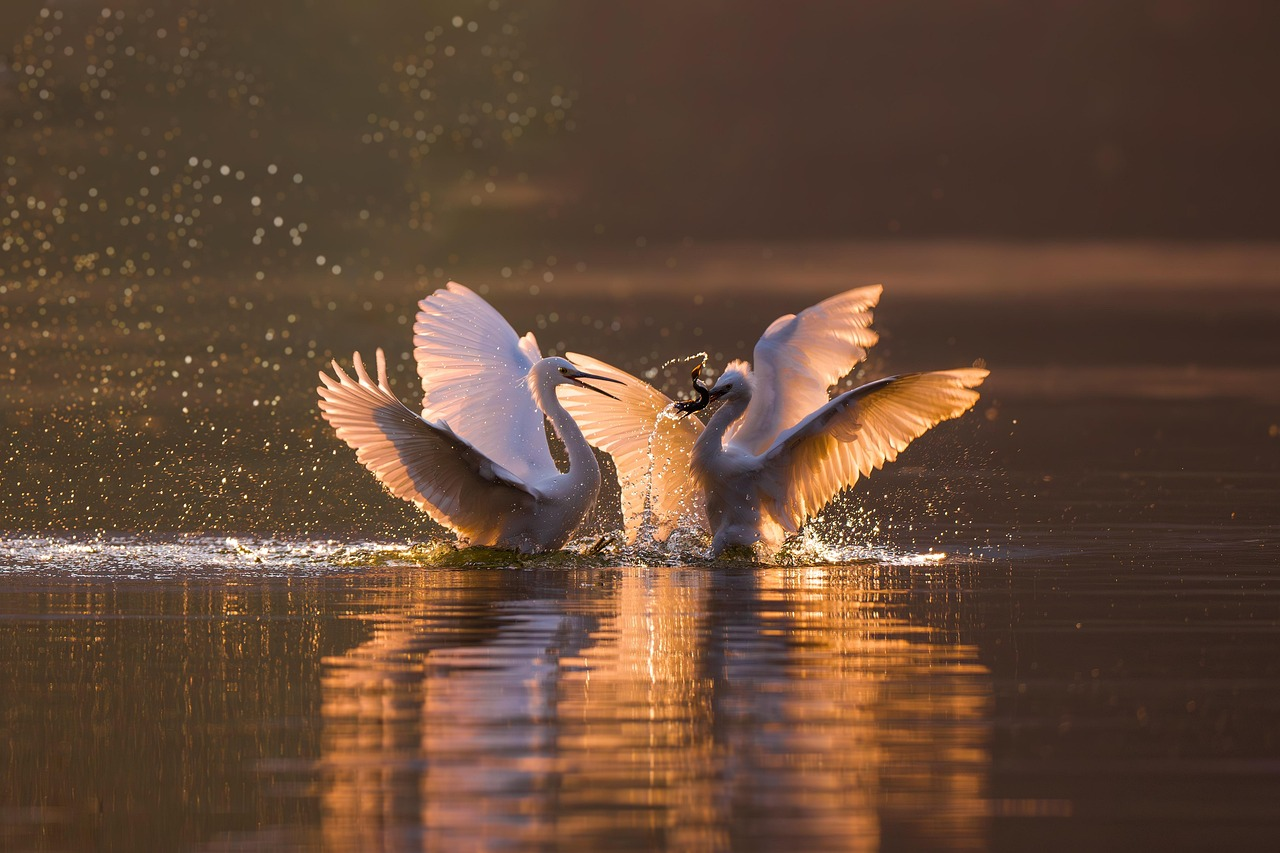
\includegraphics[width=.9\linewidth]{birds.jpg}
    \end{subplace}
\end{multiplace}

\section{Citações}

\enquote{A vida é aquilo que acontece enquanto você está ocupado fazendo outros planos} \cite{lennon}.

\Enquote{
    É uma verdade universalmente reconhecida que um homem solteiro em posse de uma grande fortuna precisa de uma esposa. Por mais pouco conhecidos os sentimentos ou pontos de vista de tal homem possam ser ao entrar numa vizinhança, esta verdade está tão bem fixada nas mentes das famílias vizinhas que ele é considerado a propriedade legítima de alguma filha sua
    \cite[][tradução por Lúcio Cardoso]{austen1813orgulho}.
}

\section{Alíneas}

\lipsum[1][1-5]:

\begin{topics}
    \item \lipsum[1][1]:
    \begin{topics}
        \item \lipsum[1][1];
        \item \lipsum[1][1];
    \end{topics}
    \item \lipsum[1][1];
    \item \lipsum[1][1]
\end{topics}

\newpage

\begin{corrprint}
    \printbibliography
\end{corrprint}

\end{document}